\documentclass[pdflatex,sn-mathphys-num,iicol]{sn-jnl}

\usepackage{graphicx}
\usepackage{amsmath,amssymb}
\usepackage{booktabs}
\usepackage{tikz}
\usetikzlibrary{arrows.meta,calc}
\setlength{\emergencystretch}{3em}
\raggedbottom

\begin{document}

\title[Self-Calibrating Control Layer for Multi-Object Trackers]{Training-Free Self-Calibrating Control Layer for Heterogeneous Multi-Object Trackers}

\author*[1]{\fnm{Ahmed Gouda} \sur{Ismail}}\email{a7medgouda1@gmail.com}
\author[1]{\fnm{Mohamed S.} \sur{Mohamed}}\email{mohamedms@mtc.edu.eg}
\author[2]{\fnm{Tarek Ahmed} \sur{Mahmoud}}\email{tarek.mohamed@eui.edu.eg}

\affil*[1]{\orgdiv{Computer Engineering and Artificial Intelligence Department}, \orgname{Military Technical College}, \orgaddress{\city{Cairo}, \country{Egypt}}}
\affil[2]{\orgdiv{Computer Engineering Department}, \orgname{Egypt University of Informatics}, \orgaddress{\city{Cairo}, \country{Egypt}}}

\abstract{Multi-object tracking pipelines are assembled from detectors and trackers developed separately, and replacing, retraining, or quantizing the detector silently shifts the confidence scale on which every tracker threshold depends. This paper presents a control layer placed between a frozen detector and a frozen tracker. The layer recalibrates itself online from the detector's own score stream with nested Otsu thresholds and estimates whether the stream is clean or noisy; on clean streams it keeps the tracker's operating point, and on noisy streams it changes which candidates the tracker receives, their scores, and the tracker's thresholds. It also supplies a continuation stage to trackers that lack one. It needs no training or dataset-specific labelled calibration, is causal, and reads only the tracker's declared operating point. One frozen configuration was evaluated unchanged on nine published trackers, four sources of detections, and three datasets, separating development from external evidence. On single-stage trackers the layer raised higher order tracking accuracy (HOTA) by 0.61 points on a predeclared external tracker and on a development tracker, with intervals above zero. When the detector confidence was halved, it restored two trackers from 0 to about 66 HOTA, and with a noisy detector it raised the multi-object tracking accuracy of two trackers by 6.0 and 7.9 points. On five two-stage trackers with well-matched detections it left HOTA unchanged or within 0.06 points. One external cell degraded significantly (1.52 HOTA points), from false noisy decisions in a short sequence. The layer costs 2.95 ms per frame on a four-core processor.}

\keywords{Multi-object tracking, Tracking by detection, Detector confidence calibration, Online adaptation, Otsu thresholding, Training-free control}

\maketitle

\section{Introduction}\label{sec:intro}
Most practical multi-object trackers work by detection: a detector scores candidate boxes in each frame, and the tracker links the boxes whose scores pass its thresholds into trajectories \cite{bewley2016sort,zhang2022bytetrack,cao2023ocsort}. In deployed systems, such as surveillance, driving, or airborne platforms \cite{miller2015multitarget,lu2024uavdetection}, the two components are rarely developed together. A detector is replaced by a faster model, retrained for a new sensor, or quantized for embedded hardware, while the tracker keeps the thresholds its authors tuned for another detector. The confidence scale of the new detector is generally different \cite{kuppers2020detcalib}, and nothing in the pipeline notices.

The consequences are large and silent. In our experiments, halving the scores of a published detector drives two well-known trackers from about 67 to 0 HOTA \cite{luiten2021hota}, because no detection reaches their fixed thresholds; a cubic reshaping of the same scores costs them about 7 and 8 points. Retuning every tracker for every detector requires labelled data from the deployment domain, which an operational system usually lacks.

This paper studies a control layer that removes that dependence without retraining or retuning. The layer sits between a frozen detector and a frozen tracker. From the recent stream of detector scores alone, it estimates how the scores separate into background, ambiguous, and confident candidates, decides whether the stream is clean enough to leave the tracker alone, and, when it is not, selects which candidates reach the tracker, remaps their scores, and moves the tracker's thresholds. The layer reads the tracker's declared operating point, called its host contract, but contains no detector, tracker, dataset, or sequence names.

The contributions are: (i) a training-free, causal layer that self-calibrates from the score stream and intervenes only when the evidence supports it; (ii) a host contract that makes it applicable to single-stage, two-stage, coordinate-only, and two-view trackers; (iii) a protocol that separates development trackers from predeclared and post-freeze external systems, with registered reproduction criteria and paired bootstrap statistics; and (iv) an evaluation of one frozen configuration that identifies where the layer helps, where it is transparent, and where it fails. The layer was designed to be detector- and tracker-agnostic and is evaluated on a heterogeneous set of published systems; the paper does not claim that it improves every tracker.

\section{Related work}\label{sec:related}
SORT \cite{bewley2016sort} predicts boxes with a Kalman filter \cite{kalman1960} and matches them to detections by overlap with the Hungarian method \cite{kuhn1955hungarian}; DeepSORT and StrongSORT add appearance \cite{wojke2017deepsort,du2023strongsort}. ByteTrack introduced a second association stage for low-confidence detections \cite{zhang2022bytetrack}, inherited by BoT-SORT \cite{aharon2022botsort}, SparseTrack \cite{liu2025sparsetrack}, BoostTrack \cite{stanojevic2024boosttrack}, and Hybrid-SORT \cite{yang2024hybridsort}. OC-SORT \cite{cao2023ocsort}, Deep OC-SORT \cite{maggiolino2023deepocsort}, and PD-SORT \cite{wang2025pdsort} use a single confidence threshold. Recent designs learn association from coordinates (C-TWiX \cite{miah2025twix}), run parallel association paths (TOPICTrack \cite{cao2025topictrack}), or associate with two detection views (TrackTrack \cite{shim2025tracktrack}); end-to-end trackers predict identities directly \cite{zeng2022motr,gao2025motip}. All of them read detector scores through fixed thresholds tuned for one detector, usually YOLOX \cite{ge2021yolox}.

Detector confidence is not calibrated across models and conditions \cite{kuppers2020detcalib}, and detectors of different families \cite{redmon2016yolo,ren2017fasterrcnn,carion2020detr,zhao2024rtdetr} produce different score distributions. Adaptive inference methods adapt computation or configuration to the input \cite{han2022dynamic,jiang2018chameleon}, but they learn or profile a policy per model. Scene-driven controllers that set a detector's operating point from image cues are tied to the detector they were calibrated with and cannot observe a change of the detector's score scale, because that change leaves the image unchanged. The layer studied here instead reads the score stream and acts on the tracker's input and thresholds.

\section{Problem formulation}\label{sec:problem}
At frame $t$ a frozen detector emits candidates $\{(\mathbf{x}_i, s_i, c_i)\}$ with boxes, scores $s_i\in(0,1)$, and class labels, down to an emission floor; $z_i=\log(s_i/(1-s_i))$ denotes the logit. A frozen tracker declares a host contract $(a, b, \ell, m_0)$: the score threshold of its first association, the lowest score from which a track can start, the lowest score any of its association stages uses, and its matching tolerance (one minus its minimum overlap). A single-stage tracker has $\ell=\min(a,b)$; a two-stage tracker has $\ell<\min(a,b)$. The layer outputs, per frame, the candidates $K_t$ passed to the tracker, their scores, and the thresholds $(a_t,b_t)$ and tolerance $m_t$ the tracker uses at that frame, from the logits of earlier frames, the current candidates, the tracker's tracks of frame $t-1$, and an optional image-motion cue. Statistics use frames before $t$ only, and frame-$t$ data enter the state after the decision. The requirements are that the layer needs no training or labelled calibration, that one frozen configuration serves every tracker, detector, and dataset, and that the output is unchanged when the tracker's operating point already fits the stream.

\section{Method}\label{sec:method}
Figure~\ref{fig:arch} summarizes the layer.

\begin{figure*}[t]
\centering
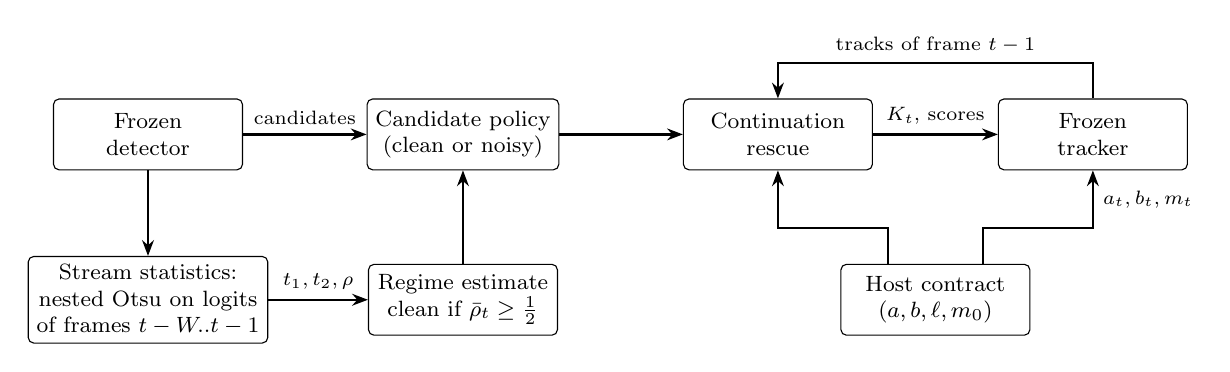
\begin{tikzpicture}[
  box/.style={draw, rounded corners=2pt, align=center, font=\footnotesize, minimum height=9mm, minimum width=24mm, inner sep=3pt},
  arr/.style={-{Stealth[length=2mm]}, thick}, lab/.style={font=\scriptsize}]
\node[box] (det) at (0,0) {Frozen\\detector};
\node[box] (pol) at (4.0,0) {Candidate policy\\(clean or noisy)};
\node[box] (res) at (8.0,0) {Continuation\\rescue};
\node[box] (trk) at (12.0,0) {Frozen\\tracker};
\node[box] (stat) at (0,-2.1) {Stream statistics:\\nested Otsu on logits\\of frames $t-W..t-1$};
\node[box] (reg) at (4.0,-2.1) {Regime estimate\\clean if $\bar\rho_t \ge \tfrac12$};
\node[box] (hc) at (10.0,-2.1) {Host contract\\$(a, b, \ell, m_0)$};
\draw[arr] (det) -- node[lab, above]{candidates} (pol);
\draw[arr] (pol) -- (res);
\draw[arr] (res) -- node[lab, above]{$K_t$, scores} (trk);
\draw[arr] (det) -- (stat);
\draw[arr] (stat) -- node[lab, above]{$t_1, t_2, \rho$} (reg);
\draw[arr] (reg) -- (pol);
\draw[arr] (hc.north) ++(-0.6,0) |- ++(0,0.45) -| (res.south);
\draw[arr] (hc.north) ++(0.6,0) |- ++(0,0.45) -| node[lab, pos=0.75, right]{$a_t, b_t, m_t$} (trk.south);
\draw[arr] (trk.north) -- ++(0,0.45) -| node[lab, pos=0.25, above]{tracks of frame $t-1$} (res.north);
\end{tikzpicture}
\caption{Self-calibrating control layer between a frozen detector and a frozen tracker. Statistics use earlier frames only; the host contract is the tracker's published operating point.}
\label{fig:arch}
\end{figure*}

\subsection{Causal self-calibration}
The layer pools the logits of all candidates of the previous $W=10$ frames and splits them twice with the exact Otsu threshold \cite{otsu1979}: $t_1$ separates background from foreground, and a second split of the foreground, $t_2$, separates ambiguous from confident candidates. The confident share of the foreground,
\begin{equation}
\rho_t = \left|\{i: z_i \ge t_2\}\right| \,/\, \left|\{i: z_i \ge t_1\}\right|,
\label{eq:rho}
\end{equation}
summarizes how cleanly the detector separates objects from clutter. Working on logits makes the splits invariant to affine transforms of the logit, such as a change of temperature. The bands are interpretable only if the stream has a background mode: when the class below $t_1$ holds fewer pooled candidates than the foreground, the first split falls inside the objects, and the frame counts as clean evidence ($\rho_t=1$). This check was added after a development diagnosis in which sequence starts with about ten candidates per frame produced splits at $t_1\approx0.6$ and $t_2\approx0.93$ in probability terms and a false noisy call.

\subsection{Intervention regimes}
The stream is clean at frame $t$ if the median $\bar\rho_t$ of $\rho$ over all past non-cold frames is at least one half, and noisy otherwise; before the first valid split the regime is cold. The regime is thus a property of the detector and scene stream, and a transient confidence dip does not flip it.

In the cold and clean regimes the tracker's thresholds are kept and lowered only as far as $t_2$ when the tracker would otherwise reject the confident class, $a_t=\min(a,\sigma(t_2))$ and likewise $b_t$, with $\sigma$ the logistic function. Scores are passed unchanged and only cross-class duplicates (one box proposed with two class labels) are removed. On a stream whose confident class lies above the tracker's thresholds, the tracker receives exactly its native input.

In the noisy regime the primary band $z\ge t_2$ may start and continue tracks, the extension band $t_1\le z<t_2$ may only continue them, and candidates below $t_1$ are discarded. Scores are remapped through their empirical distribution in the stream, primary candidates to $[0.5,1)$ and extension candidates to $[0.1,0.5)$, and the tracker's association and birth thresholds are set to 0.5. Duplicates are resolved with track context: a weaker candidate overlapping a stronger one by more than one half is removed unless a different track of the previous frame claims it, which keeps occluded people in crowds.

\subsection{Continuation rescue and motion rule}
A foreground candidate that continues an existing track of frame $t-1$ with overlap at least one half, where no usable candidate covers that track and the tracker could not see the candidate at the operating point passed this frame, is passed with its score raised just above the lowest threshold the tracker uses at that frame. For a two-stage tracker this set is empty by construction; for a single-stage tracker it supplies the missing continuation stage. In noisy frames only, and only when an image-motion cue is available, the matching tolerance widens with the ratio $r_t$ of the current global motion (phase correlation on a quarter-resolution frame \cite{reddy1996phasecorr}) to its past median: $m_t=\min\left(0.95,\,1-(1-m_0)/\max(1,r_t)\right)$.

\subsection{Host contract and cost}
Table~\ref{tab:contracts} lists the contracts; each value is a documented property of the published configuration. An adapter per tracker family maps the decision onto the tracker's interface, and the authors' post-processing (interpolation, offline linking) is kept unchanged. With $n$ candidates per frame and $k$ tracks, the cost is $O(Wn\log(Wn)+n^2+nk)$ plus one phase correlation.

\begin{table*}[t]
\centering
\caption{Host contracts: the operating point each published tracker declares, as used by the layer. $\tau$ is the tracker's own published threshold, which differs between trackers and, for TrackTrack, between sequences.}
\label{tab:contracts}
\footnotesize
\begin{tabular}{p{3.4cm}cccccp{3.6cm}}
\hline
Tracker (setting) & Type & assoc & birth & low & match & Decision mapped to \\
\hline
ByteTrack (official MOT17) & two-stage & 0.6 & 0.7 & 0.1 & 0.8 & thresholds, candidates, scores \\
ByteTrack (library default) & two-stage & 0.25 & 0.25 & 0.1 & 0.8 & same \\
SparseTrack & two-stage & $\tau$ & $\tau+0.1$ & 0.1 & published & same \\
BoostTrack & two-stage & $\tau$ & $\tau$ & 0.1 & $1-$IoU gate & same \\
Hybrid-SORT & two-stage & $\tau$ & $\tau$ & 0.1 & $1-$IoU gate & same \\
OC-SORT & single-stage & 0.6 & 0.6 & 0.6 & 0.7 & same \\
PD-SORT & single-stage & $\tau$ & $\tau$ & $\tau$ & $1-$IoU gate & same \\
C-TWiX (MOT17 / KITTI / DanceTrack) & single-stage & 0.5 & 0.7 / 0.5 / 0.9 & 0.5 & not mapped & candidates, scores, two score thresholds \\
TrackTrack & two-view & $\tau_{\mathrm{det}}$ & $\tau_{\mathrm{init}}$ & 0.1 & not mapped & candidates in both views, two thresholds \\
\botrule
\end{tabular}
\end{table*}


\section{Development and evaluation protocol}\label{sec:protocol}
The layer evolved from an earlier design that always intervened. That design helped with miscalibrated and noisy detectors but degraded strong published trackers on MOT17: SparseTrack by 4.15 HOTA ($[-5.54,-1.66]$) and BoostTrack by 5.89 ($[-7.76,-2.87]$), because overlap-based duplicate removal deleted occluded people and its thresholds were stricter than the trackers' own (false negatives rose by 4,955 and 6,167). The regime estimate, the self-limiting clean regime, track-context duplicates, the whole-stream regime, the interpretability check, and the rescue were each introduced to remove a diagnosed failure. On development data, emulating the prior design reduced ByteTrack from 67.70 to 56.41 HOTA; the regime and clean-regime changes restored SparseTrack from 64.72 to 68.93 and BoostTrack from 62.61 to 68.37; the rescue added 0.2--0.4 points for OC-SORT. Four variants were rejected on evidence, including rescuing below a two-stage tracker's low stage (+700 to +1000 false positives) and remapping scores in clean frames (up to $-1.6$ HOTA).

The configuration was then frozen, recorded in a version-control tag, and protected by a lock file of hashes of the layer, its configuration, and the runners, verified before every later run; 61 automated tests check causality, state reset, pass-through, name independence, and lock integrity. Development cells (MOT17 val-half \cite{milan2016mot16} with four trackers, KITTI tracking \cite{geiger2012kitti} with three trackers and two detectors, score-transform stress tests) were visible during design. PD-SORT and Hybrid-SORT were declared before being run and were run once. C-TWiX, TrackTrack, and TOPICTrack were run after the freeze under a registered protocol that fixed host contracts, reproduction criteria (EXACT: within 0.2 HOTA of the authors' number; CLOSE: within 1.0 with a documented, untuned cause), and predictions. Both arms of every comparison use the same detections and environment; 95\% intervals come from a percentile bootstrap over sequences with 10,000 resamples and seed 42 \cite{efron1993bootstrap}; ties are $|\Delta\mathrm{HOTA}|<0.01$. Metrics are HOTA \cite{luiten2021hota}, MOTA \cite{bernardin2008clear}, and IDF1 \cite{ristani2016idf1}, computed with the TrackEval library (commit 12c8791) following MOTChallenge practice \cite{dendorfer2021motchallenge}.

\section{Results}\label{sec:results}
Figure~\ref{fig:forest} summarizes every cell.

\begin{figure}[t]
\centering
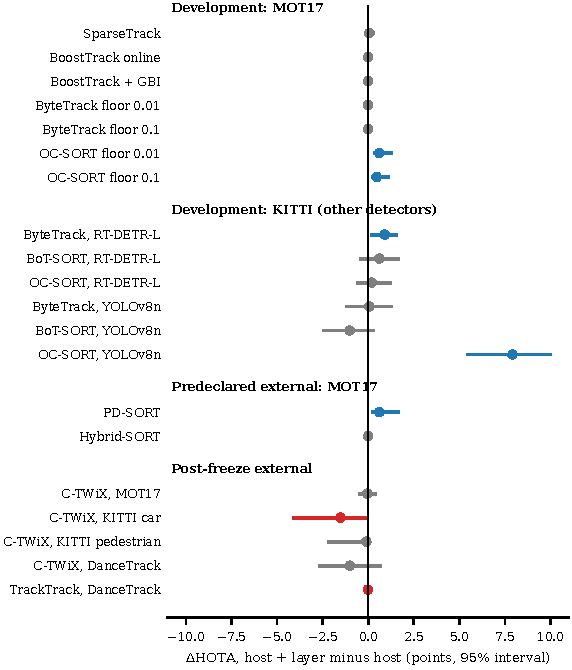
\includegraphics[width=\columnwidth]{figures/fig3_forest_col.pdf}
\caption{Difference in HOTA (tracker with the frozen layer minus tracker alone) with 95\% paired-bootstrap interval for every evaluated cell. Blue: above zero; red: below zero; gray: includes zero or identical output.}
\label{fig:forest}
\end{figure}

\subsection{Tracker transfer}
Table~\ref{tab:mot17} gives the development trackers on MOT17 val-half. The two-stage trackers with well-matched detections were left unchanged: BoostTrack and ByteTrack at floor 0.1 produced identical output, ByteTrack at floor 0.01 changed by $-0.014$ and SparseTrack by $+0.06$, both with intervals including zero. This is the intended self-limiting behavior, which the prior design lacked. The single-stage OC-SORT improved at both emission floors, by $+0.61$ ($[+0.36,+1.24]$) and $+0.46$ ($[+0.27,+1.09]$) HOTA and about 1.3 MOTA, on 7 of 7 sequences in both settings, through the continuation rescue.

\begin{table*}[t]
\centering
\caption{Development hosts on MOT17 val-half (published YOLOX-X detections). Host = our reproduction; $\Delta$ = host with the frozen layer minus host, with 95\% paired-bootstrap interval (10,000 resamples, seed 42); bold intervals exclude zero. The floor is the lowest detector score emitted.}
\label{tab:mot17}
\footnotesize
\resizebox{\textwidth}{!}{%
\begin{tabular}{llllccc}
\hline
Tracker & Setting & Paper HOTA / MOTA / IDF1 & Host HOTA / MOTA / IDF1 & $\Delta$HOTA & $\Delta$MOTA & $\Delta$IDF1 \\
\hline
SparseTrack & -- & 69.2 / 76.8 / 81.4 & 68.88 / 77.85 / 81.97 & $+0.06$ [$-0.01$, $+0.25$] & $+0.08$ [$-0.03$, $+0.30$] & $+0.16$ [$-0.01$, $+0.70$] \\
BoostTrack & online & 68.37 / 75.56 / 81.35 & 68.49 / 75.50 / 81.41 & 0 (identical) & 0 (identical) & 0 (identical) \\
BoostTrack & + GBI & 71.33 / 80.55 / 83.84 & 71.72 / 81.03 / 84.16 & 0 (identical) & 0 (identical) & 0 (identical) \\
ByteTrack & floor 0.01 & -- / 76.6 / 79.3 & 67.70 / 77.60 / 79.47 & $-0.014$ [$-0.058$, $+0.009$] & $+0.06$ [$-0.15$, $+0.34$] & $-0.03$ [$-0.14$, $+0.04$] \\
ByteTrack & floor 0.1 & -- / 76.6 / 79.3 & 67.70 / 77.60 / 79.47 & 0 (identical) & 0 (identical) & 0 (identical) \\
OC-SORT & floor 0.01 & 66.5 / 74.9 / 77.7 & 66.43 / 74.67 / 78.05 & {\boldmath $+0.61$ [$+0.36$, $+1.24$]} & {\boldmath $+1.27$ [$+0.17$, $+3.01$]} & $+0.66$ [$-0.25$, $+1.60$] \\
OC-SORT & floor 0.1 & 66.5 / 74.9 / 77.7 & 66.44 / 74.67 / 78.05 & {\boldmath $+0.46$ [$+0.27$, $+1.09$]} & {\boldmath $+1.26$ [$+0.37$, $+3.34$]} & {\boldmath $+0.287$ [$+0.003$, $+0.838$]} \\
\botrule
\end{tabular}}
\end{table*}


\subsection{Detector change and confidence shift}
On KITTI (Table~\ref{tab:kitti}), the noisy RT-DETR-L stream \cite{zhao2024rtdetr} gave two-stage trackers large MOTA and IDF1 gains: ByteTrack $+5.98$ MOTA ($[+1.16,+9.94]$) and $+0.91$ HOTA ($[+0.22,+1.55]$), BoT-SORT $+7.86$ MOTA ($[+2.21,+13.44]$). With YOLOv8n, OC-SORT gained 7.91 HOTA ($[+5.47,+9.98]$), while ByteTrack and BoT-SORT lost 1.87 and 2.43 MOTA (the latter significant) with about half as many identity switches (Section~\ref{sec:analysis}).

\begin{table*}[t]
\centering
\caption{Detector transfer on KITTI tracking training (official HOTA, car and pedestrian averaged). BoT-SORT excludes one sequence on which the unmodified tracker fails numerically.}
\label{tab:kitti}
\footnotesize
\resizebox{\textwidth}{!}{%
\begin{tabular}{llcccc}
\hline
Tracker & Detector & Host HOTA / MOTA / IDF1 & $\Delta$HOTA & $\Delta$MOTA & $\Delta$IDF1 \\
\hline
ByteTrack & RT-DETR-L & 50.73 / 47.27 / 64.98 & {\boldmath $+0.91$ [$+0.22$, $+1.55$]} & {\boldmath $+5.98$ [$+1.16$, $+9.94$]} & {\boldmath $+3.87$ [$+1.67$, $+5.06$]} \\
BoT-SORT & RT-DETR-L & 53.91 / 48.25 / 67.74 & $+0.61$ [$-0.39$, $+1.61$] & {\boldmath $+7.86$ [$+2.21$, $+13.44$]} & {\boldmath $+3.10$ [$+1.00$, $+4.57$]} \\
OC-SORT & RT-DETR-L & 52.64 / 57.59 / 69.87 & $+0.19$ [$-0.57$, $+1.19$] & $-0.57$ [$-4.36$, $+1.40$] & $+0.04$ [$-1.31$, $+1.78$] \\
ByteTrack & YOLOv8n & 45.31 / 46.54 / 60.92 & $+0.06$ [$-1.19$, $+1.24$] & $-1.87$ [$-6.25$, $+0.03$] & $+1.49$ [$-0.36$, $+3.27$] \\
BoT-SORT & YOLOv8n & 49.21 / 49.89 / 64.41 & $-1.02$ [$-2.43$, $+0.25$] & {\boldmath $-2.43$ [$-7.43$, $-0.14$]} & $+0.35$ [$-2.10$, $+2.27$] \\
OC-SORT & YOLOv8n & 36.27 / 33.99 / 50.46 & {\boldmath $+7.91$ [$+5.47$, $+9.98$]} & {\boldmath $+9.40$ [$+1.10$, $+12.30$]} & {\boldmath $+9.60$ [$+5.61$, $+12.16$]} \\
\botrule
\end{tabular}}
\end{table*}


To isolate calibration, the published MOT17 detections were transformed by four monotone maps before the tracker, whose thresholds stayed fixed (Fig.~\ref{fig:shift}). Halving the scores drove ByteTrack (official setting) and OC-SORT to 0 HOTA; with the layer they reached 66.17 and 66.72. Cubing reduced them to 60.92 and 58.34, restored to 65.81 and 66.60, and BoostTrack went from 61.33 to 64.84. The ByteTrack library setting, whose low thresholds already admit the shifted scores, changed by at most 0.14 points. These are development cells reported without intervals.

\begin{figure*}[t]
\centering
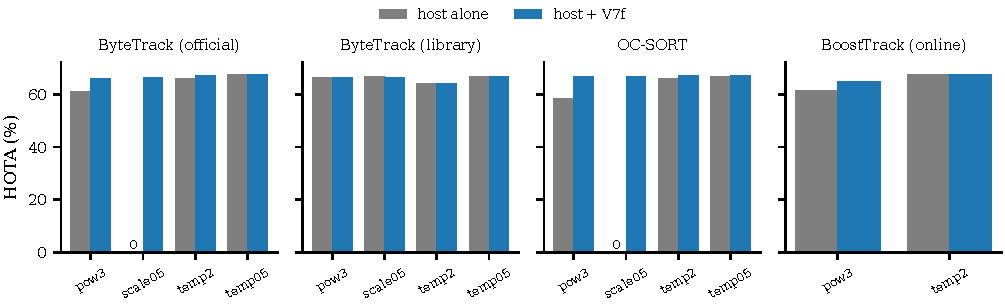
\includegraphics[width=0.9\textwidth]{figures/fig5_calibration_shift.pdf}
\caption{Detector confidence shift on MOT17 val-half: HOTA of each published tracker with its published thresholds, alone and with the frozen layer, after four monotone transforms of the detector scores.}
\label{fig:shift}
\end{figure*}

\subsection{External systems}
Table~\ref{tab:external} gives every external system. PD-SORT \cite{wang2025pdsort}, reproduced identically to the authors' released output, improved by 0.61 HOTA ($[+0.27,+1.65]$), 1.13 MOTA, and 0.82 IDF1, all intervals above zero, on 7 of 7 sequences; false negatives fell by 1,291 and false positives rose by 681. Hybrid-SORT \cite{yang2024hybridsort}, two-stage, produced identical output, as predicted. After the freeze, C-TWiX \cite{miah2025twix} changed by $-0.05$ HOTA on MOT17, $-0.10$ on KITTI pedestrians, and $-1.00$ on DanceTrack \cite{sun2022dancetrack}, all with intervals including zero, and lost 1.52 ($[-4.05,-0.13]$) on KITTI cars. TrackTrack \cite{shim2025tracktrack} changed by $-0.013$ ($[-0.032,-0.001]$), significant but negligible, with 21 of 25 sequences tied. TOPICTrack \cite{cao2025topictrack} failed the reproduction criterion (67.54 against 69.6) and is excluded.

\begin{table*}[t]
\centering
\caption{External systems evaluated once with the frozen layer. Reproduction class against the authors' reported number (EXACT: $|\Delta\mathrm{HOTA}|\le0.2$; CLOSE: $\le1.0$ with a documented, untuned cause). TOPICTrack failed reproduction and is excluded from the analysis.}
\label{tab:external}
\footnotesize
\resizebox{\textwidth}{!}{%
\begin{tabular}{llllccc}
\hline
System & Data & Reference / reproduced HOTA & Class & $\Delta$HOTA & $\Delta$MOTA & $\Delta$IDF1 \\
\hline
\multicolumn{7}{l}{\textit{Predeclared before the runs}}\\
PD-SORT & MOT17 val-half & 68.01 / 68.01 & EXACT (released output) & {\boldmath $+0.61$ [$+0.27$, $+1.65$]} & {\boldmath $+1.13$ [$+0.27$, $+3.03$]} & {\boldmath $+0.82$ [$+0.43$, $+1.94$]} \\
Hybrid-SORT & MOT17 val-half & 67.1 / 66.70 & CLOSE & 0 (identical) & 0 (identical) & 0 (identical) \\
\multicolumn{7}{l}{\textit{Post-freeze, protocol registered before the runs}}\\
C-TWiX & MOT17 val-half & 77.8 / 77.55 & CLOSE & $-0.05$ [$-0.46$, $+0.40$] & $+0.24$ [$-0.58$, $+1.12$] & $+0.18$ [$-0.47$, $+1.14$] \\
C-TWiX (car) & KITTI MOTS val & 89.3 / 89.27 & EXACT & {\boldmath $-1.52$ [$-4.05$, $-0.13$]} & {\boldmath $-2.11$ [$-5.89$, $-0.17$]} & {\boldmath $-1.21$ [$-3.32$, $-0.10$]} \\
C-TWiX (pedestrian) & KITTI MOTS val & 71.4 / 70.77 & CLOSE & $-0.10$ [$-2.16$, $+0.03$] & $-0.31$ [$-4.86$, $+0.10$] & $-0.01$ [$-1.90$, $+0.08$] \\
C-TWiX & DanceTrack val & 60.4 / 59.62 & CLOSE & $-1.00$ [$-2.62$, $+0.65$] & $+0.13$ [$-0.39$, $+0.47$] & $-1.55$ [$-3.76$, $+0.52$] \\
TOPICTrack & MOT17 val-half & 69.6 / 67.54 & FAILED & \multicolumn{3}{c}{not analyzed} \\
TrackTrack & DanceTrack val & 63.3 / 62.96 & CLOSE & {\boldmath $-0.013$ [$-0.032$, $-0.001$]} & {\boldmath $-0.073$ [$-0.208$, $-0.004$]} & $+0.009$ [$-0.001$, $+0.028$] \\
\botrule
\end{tabular}}
\end{table*}


\section{Analysis}\label{sec:analysis}
\textit{When the layer acts.} The direction of the effect follows two properties of the pipeline rather than the dataset: whether the tracker has a continuation stage, and whether the detector's score distribution matches the tracker's thresholds. On the post-freeze streams, 99.7\% of MOT17 frames and 99.9\% of DanceTrack frames were classified clean (Fig.~\ref{fig:regimes}a), and those pipelines stayed at or near their native output. Of the 16 cells with an interval in Fig.~\ref{fig:forest}, 5 are above zero, 2 below, and 9 include zero; 4 further cells are identical.

\begin{figure*}[t]
\centering
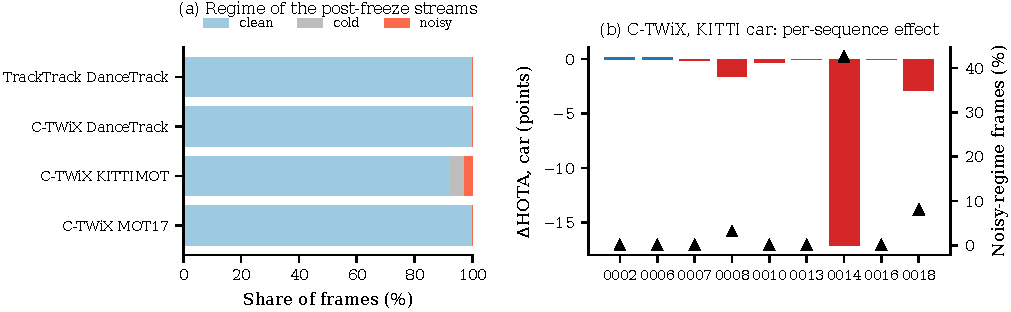
\includegraphics[width=0.9\textwidth]{figures/fig6_regimes_failure.pdf}
\caption{(a) Share of frames in each regime on the post-freeze streams. (b) C-TWiX on KITTI cars: per-sequence HOTA difference (bars) and share of frames classified noisy (triangles).}
\label{fig:regimes}
\end{figure*}

\textit{Failure cases.} The external loss on KITTI cars is concentrated in one sequence: in sequence 0014 the layer classified 45 of 106 frames as noisy and HOTA fell by 17.09 points, while six of the other eight sequences changed by less than 0.4 (Fig.~\ref{fig:regimes}b). In this short sequence the whole-stream median of $\rho$ had little history, and the noisy bands most likely removed detections the coordinate-based association relies on. A cold-start protection that requires a minimum history before a noisy decision is a natural remedy and is left to future work. With the under-confident YOLOv8n on KITTI ($\rho\approx0.45$), the noisy rule that only the primary band may start tracks removed true births for ByteTrack and BoT-SORT; a host-relative band that fixed this let false tracks through on a noisy aerial stream and was rejected. On DanceTrack, C-TWiX lost 1.00 HOTA with two sequences losing more than 10 points while the regime was clean, so the clean-regime operations interact with its learned association; which operation causes the loss was not isolated.

\textit{Runtime.} On a four-core Intel Xeon without a graphics processor, with live YOLOv8n (736 pixels) and ByteTrack on three KITTI sequences, the layer took 2.95 ms per frame (4.39 ms at the 95th percentile, including the motion cue); end-to-end time rose from 57.85 to 60.44 ms (4.5\%), and the tracker became faster (2.04 to 1.43 ms) because it received fewer candidates. The detector dominates, and no throughput is claimed for other hardware.

\textit{Limitations.} Most gains are development evidence; among external systems only PD-SORT improved. External systems were evaluated on validation splits with released detections, reproductions run on central processing units differ from the authors' numbers by up to 0.8 HOTA, the motion rule could not be tested on external systems, and no embedded hardware was measured.

\section{Conclusion}\label{sec:conclusion}
A training-free layer that self-calibrates from a detector's score stream and adapts a frozen tracker through a declared host contract was evaluated with one frozen configuration on nine published trackers. It improved single-stage trackers, including a predeclared external one; it restored trackers whose thresholds no longer matched a shifted confidence scale; it raised the MOTA of two-stage trackers with a noisy detector; and it left well-matched two-stage pipelines unchanged, removing the degradation of the prior design. It failed on a short stream where false noisy decisions cost one external tracker 1.52 HOTA points, and on an under-confident detector with low-threshold trackers.

\backmatter

\bmhead{Acknowledgements}
The authors thank the authors of the evaluated trackers for releasing their code, weights, and detections, and the maintainers of MOT17, KITTI, DanceTrack, and TrackEval.

\section*{Declarations}

\noindent\textbf{Funding:} The authors declare that no funds, grants, or other support were received during the preparation of this manuscript.

\noindent\textbf{Competing interests:} The authors have no relevant financial or non-financial interests to disclose.

\noindent\textbf{Ethics approval and consent to participate:} Not applicable.

\noindent\textbf{Consent for publication:} Not applicable.

\noindent\textbf{Data availability:} All datasets used (MOT17, KITTI tracking, DanceTrack) are publicly available from their providers. Tracker outputs, bootstrap records, and the frozen configuration are available from the corresponding author on reasonable request.

\noindent\textbf{Materials availability:} Not applicable.

\noindent\textbf{Code availability:} The implementation of the layer and the evaluation scripts are available from the corresponding author on reasonable request.

\noindent\textbf{Author contribution:} Ahmed Gouda Ismail: conceptualization, methodology, software, experiments, formal analysis, writing of the original draft. Mohamed S. Mohamed and Tarek Ahmed Mahmoud: supervision, methodology review, writing (review and editing). All authors read and approved the final manuscript.

\bibliography{references}

\end{document}
